% Fig. 2 -- The Intentions Game and its models (Sections 4.1-4.2). Pure TikZ; build: xelatex.
% (A) Task timeline with what each part measures; (B) the model space: partner representation x
% direction of self-other transfer. New models (H, I, C) are shaded. No hue (reserved for entities).
\documentclass[border=0pt]{standalone}
% figstyle.tex -- shared style for all figures of "Epistemic Trust as Inference About Other Minds".
% Compile each figure with xelatex (standalone class). Full-width figures are exactly 504pt wide,
% the \textwidth of the Frontiers template, so they are included at 100% and never rescaled.
%
% Colour roles (validated with the dataviz skill's validate_palette.js on a white surface):
%   groups   : controls = slot 1 blue #2a78d6, BPD = slot 2 orange #eb6834 (all-pairs PASS)
%   stances  : trusting = green #008300, mistrusting = violet #6250d6 (all-pairs PASS; tritan 7.6,
%              so always paired with a second cue: dash for rigid stances, plus labels)
%   models   : theoretical curves in primary ink (no hue, so hues stay reserved for entities)
%   chrome   : ink #0b0b0b / #52514e / #898781, gridline #e1e0d9, axis #c3c2b7 (reference palette)

\usepackage{fontspec}
% Fonts are loaded by file name: XeTeX then finds them in TeX Live without system registration.
\setmainfont{texgyreheros}[Extension=.otf, UprightFont=*-regular, BoldFont=*-bold,
  ItalicFont=*-italic, BoldItalicFont=*-bolditalic]
\setsansfont{texgyreheros}[Extension=.otf, UprightFont=*-regular, BoldFont=*-bold,
  ItalicFont=*-italic, BoldItalicFont=*-bolditalic]
\renewcommand{\familydefault}{\sfdefault}
\hyphenpenalty=10000 \exhyphenpenalty=10000   % figures never hyphenate
\usepackage{unicode-math}
\setmathfont{FiraMath-Regular.otf}[Scale=MatchLowercase]   % sans-serif math to match the text

\usepackage{tikz}
\usetikzlibrary{positioning,calc,fit,backgrounds,arrows.meta}
\usepackage{pgfplots}
\pgfplotsset{compat=1.18}
\usepgfplotslibrary{groupplots,fillbetween}

% ---- colours ---------------------------------------------------------------
\definecolor{inkPrimary}{HTML}{0B0B0B}
\definecolor{inkSecondary}{HTML}{52514E}
\definecolor{inkMuted}{HTML}{898781}
\definecolor{gridLine}{HTML}{E1E0D9}
\definecolor{axisLine}{HTML}{C3C2B7}
\definecolor{bandFill}{HTML}{F0EFEC}
\definecolor{groupControls}{HTML}{2A78D6}
\definecolor{groupBPD}{HTML}{EB6834}
\definecolor{stanceTrust}{HTML}{008300}
\definecolor{stanceMistrust}{HTML}{6250D6}

% ---- type sizes (true size: figures are never rescaled) --------------------
\newcommand{\figfont}{\fontsize{8}{9.6}\selectfont}
\newcommand{\ticksize}{\fontsize{7}{8.4}\selectfont}
\newcommand{\panelfont}{\fontsize{9}{10.8}\selectfont\bfseries}

% ---- line weights -----------------------------------------------------------
\tikzset{
  hairline/.style={line width=0.4pt},
  dataline/.style={line width=1.3pt, line cap=round, line join=round},
  rigid/.style={dash pattern=on 3.2pt off 2.2pt},
  panel label/.style={font=\panelfont, text=inkPrimary, anchor=north west, inner sep=0pt},
  note/.style={font=\ticksize, text=inkSecondary, inner sep=1pt},
}

% ---- row filter: plot only the rows whose column #1 equals #2 (e.g. group = BPD) ----
\pgfplotsset{
  only rows/.style 2 args={
    unbounded coords=discard,
    x filter/.append code={%
      \edef\figRowValue{\thisrow{#1}}\edef\figWanted{#2}%
      \ifx\figRowValue\figWanted\else\def\pgfmathresult{inf}\fi},
  },
  group dots/.style={only marks, mark=*, mark size=1.75pt,
    mark options={draw=white, line width=0.5pt, fill=#1}, color=#1},
}

% ---- the shared axis style --------------------------------------------------
\pgfplotsset{
  paper axis/.style={
    scale only axis,
    axis lines*=left,
    axis line style={axisLine, line width=0.4pt},
    every tick/.style={axisLine, line width=0.4pt},
    tick align=outside,
    major tick length=2.5pt,
    minor tick length=1.5pt,
    tick label style={font=\ticksize, text=inkSecondary},
    label style={font=\figfont, text=inkPrimary},
    title style={font=\figfont, text=inkPrimary, align=center},
    grid=major,
    major grid style={gridLine, line width=0.4pt},
    clip mode=individual,
    legend style={draw=none, fill=none, font=\ticksize, text=inkSecondary},
    legend cell align=left,
    every axis plot/.append style={dataline},
  },
}

\newcommand{\sub}{\ticksize\color{inkSecondary}}
\tikzset{
  phase/.style={draw=axisLine, line width=0.5pt, fill=white, rounded corners=3pt, align=center,
                font=\figfont, text=inkPrimary, inner sep=4pt, minimum height=40pt, anchor=west},
  flow/.style={-{Stealth[length=4pt, width=3.6pt]}, line width=0.7pt, draw=inkSecondary},
  measure/.style={font=\ticksize, text=inkSecondary, align=center, anchor=north, inner sep=1pt},
  model/.style={draw=axisLine, line width=0.5pt, fill=white, rounded corners=2.5pt, font=\figfont,
                text=inkPrimary, inner sep=2.5pt, minimum width=24pt, minimum height=15pt},
  newmodel/.style={model, draw=inkPrimary, fill=bandFill, line width=0.7pt},
  newtag/.style={font=\fontsize{6}{7}\selectfont, text=inkSecondary, anchor=south west, inner sep=0.5pt},
  colhead/.style={font=\figfont, text=inkPrimary, align=center, anchor=south, inner sep=1pt},
  rowhead/.style={font=\figfont, text=inkPrimary, align=left, anchor=west, inner sep=1pt},
  cell/.style={draw=gridLine, line width=0.5pt},
}

\begin{document}
\figfont
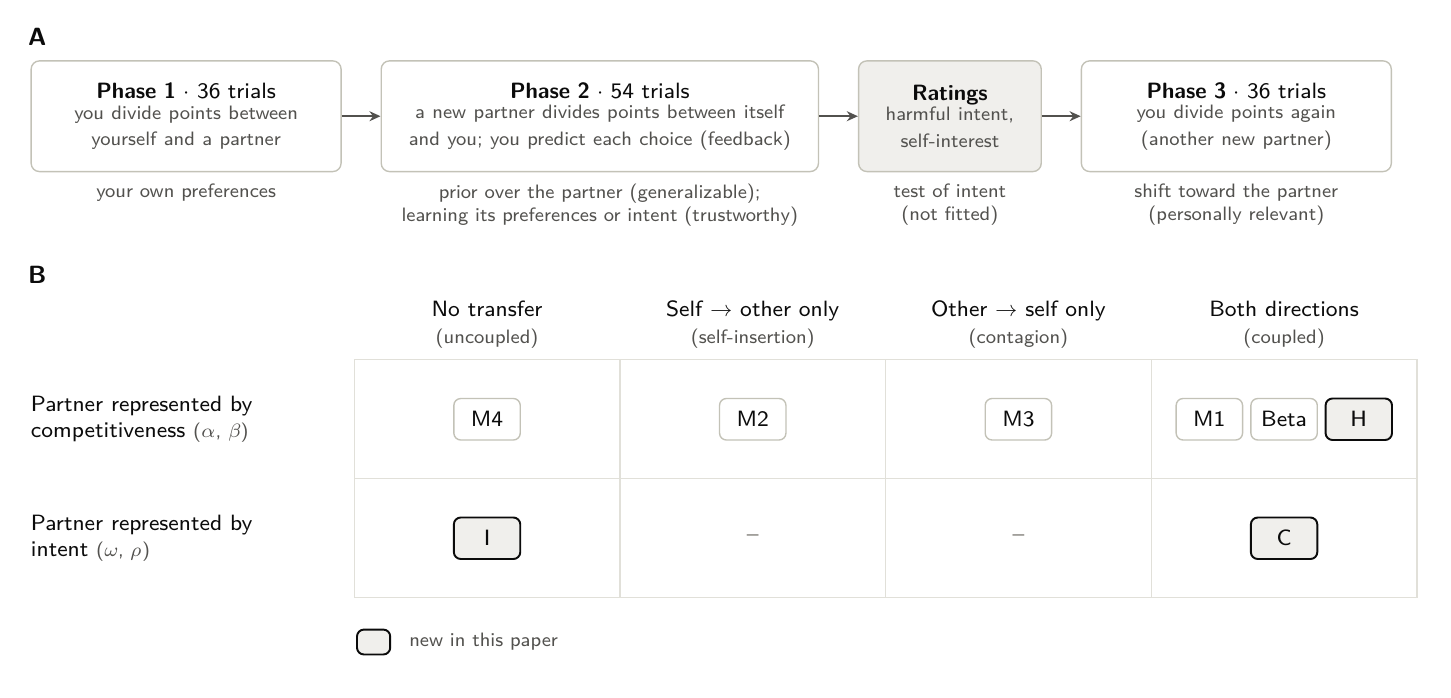
\begin{tikzpicture}
  \useasboundingbox (0,0) rectangle (504pt,232pt);

  % ======================= A: the task =======================
  \node[phase, text width=104pt] (p1) at (1pt,200pt)
    {\textbf{Phase 1} \(\cdot\) 36 trials\\[-1pt]{\sub you divide points between\\yourself and a partner}};
  \node[phase, text width=150pt] (p2) at ([xshift=14pt]p1.east)
    {\textbf{Phase 2} \(\cdot\) 54 trials\\[-1pt]{\sub a new partner divides points between itself\\and you; you predict each choice (feedback)}};
  \node[phase, text width=58pt, fill=bandFill] (r) at ([xshift=14pt]p2.east)
    {\textbf{Ratings}\\[-1pt]{\sub harmful intent,\\self-interest}};
  \node[phase, text width=104pt] (p3) at ([xshift=14pt]r.east)
    {\textbf{Phase 3} \(\cdot\) 36 trials\\[-1pt]{\sub you divide points again\\(another new partner)}};
  \draw[flow] (p1) -- (p2);  \draw[flow] (p2) -- (r);  \draw[flow] (r) -- (p3);

  \node[measure] at ([yshift=-3pt]p1.south) {your own preferences};
  \node[measure] at ([yshift=-3pt]p2.south) {prior over the partner (generalizable);\\learning its preferences or intent (trustworthy)};
  \node[measure] at ([yshift=-3pt]r.south) {test of intent\\(not fitted)};
  \node[measure] at ([yshift=-3pt]p3.south) {shift toward the partner\\(personally relevant)};

  % ======================= B: the model space =======================
  % grid geometry: row-header column 0..118pt; four columns of 96.5pt; rows of 44pt
  \def\xa{118pt}\def\cw{96pt}
  \def\yTop{112pt}\def\yMid{69pt}\def\yBot{26pt}
  % cells
  \foreach \c in {0,1,2,3} {
    \draw[cell] ($(\xa,\yTop)+(\c*\cw,0)$) rectangle ($(\xa,\yMid)+(\c*\cw+\cw,0)$);
    \draw[cell] ($(\xa,\yMid)+(\c*\cw,0)$) rectangle ($(\xa,\yBot)+(\c*\cw+\cw,0)$);
  }
  % column headers
  \node[colhead] at ($(\xa,\yTop)+(0.5*\cw,3pt)$) {No transfer\\{\sub (uncoupled)}};
  \node[colhead] at ($(\xa,\yTop)+(1.5*\cw,3pt)$) {Self \(\rightarrow\) other only\\{\sub (self-insertion)}};
  \node[colhead] at ($(\xa,\yTop)+(2.5*\cw,3pt)$) {Other \(\rightarrow\) self only\\{\sub (contagion)}};
  \node[colhead] at ($(\xa,\yTop)+(3.5*\cw,3pt)$) {Both directions\\{\sub (coupled)}};
  % row headers
  \node[rowhead] at (0pt,90.5pt) {Partner represented by\\competitiveness {\sub (\(\alpha\), \(\beta\))}};
  \node[rowhead] at (0pt,47.5pt)  {Partner represented by\\intent {\sub (\(\omega\), \(\rho\))}};

  % competitiveness row
  \node[model] at ($(\xa,90.5pt)+(0.5*\cw,0)$) {M4};
  \node[model] at ($(\xa,90.5pt)+(1.5*\cw,0)$) {M2};
  \node[model] at ($(\xa,90.5pt)+(2.5*\cw,0)$) {M3};
  \node[model]    (m1) at ($(\xa,90.5pt)+(3.5*\cw-27pt,0)$) {M1};
  \node[model]    (mb) at ($(\xa,90.5pt)+(3.5*\cw,0)$) {Beta};
  \node[newmodel] (mh) at ($(\xa,90.5pt)+(3.5*\cw+27pt,0)$) {H};
  % intent row
  \node[newmodel] (mi) at ($(\xa,47.5pt)+(0.5*\cw,0)$) {I};
  \node[font=\figfont, text=inkMuted] at ($(\xa,47.5pt)+(1.5*\cw,0)$) {--};
  \node[font=\figfont, text=inkMuted] at ($(\xa,47.5pt)+(2.5*\cw,0)$) {--};
  \node[newmodel] (mc) at ($(\xa,47.5pt)+(3.5*\cw,0)$) {C};

  % key
  \node[newmodel, minimum width=12pt, minimum height=9pt, inner sep=0pt] (key) at (125pt,10pt) {};
  \node[font=\ticksize, text=inkSecondary, anchor=west] at ([xshift=3pt]key.east) {new in this paper};

  % ======================= panel letters =======================
  \node[panel label] at (0pt,232pt) {A};
  \node[panel label] at (0pt,146pt) {B};
\end{tikzpicture}
\end{document}
